\documentclass[border=10pt]{standalone}
\usepackage[svgnames]{xcolor}
\usepackage{amsmath}
\usepackage{pgfplots}
\pgfplotsset{compat=newest}
\usepackage[sfdefault]{FiraSans}
\usepackage{FiraMono}
\renewcommand*\familydefault{\sfdefault}
\begin{document}
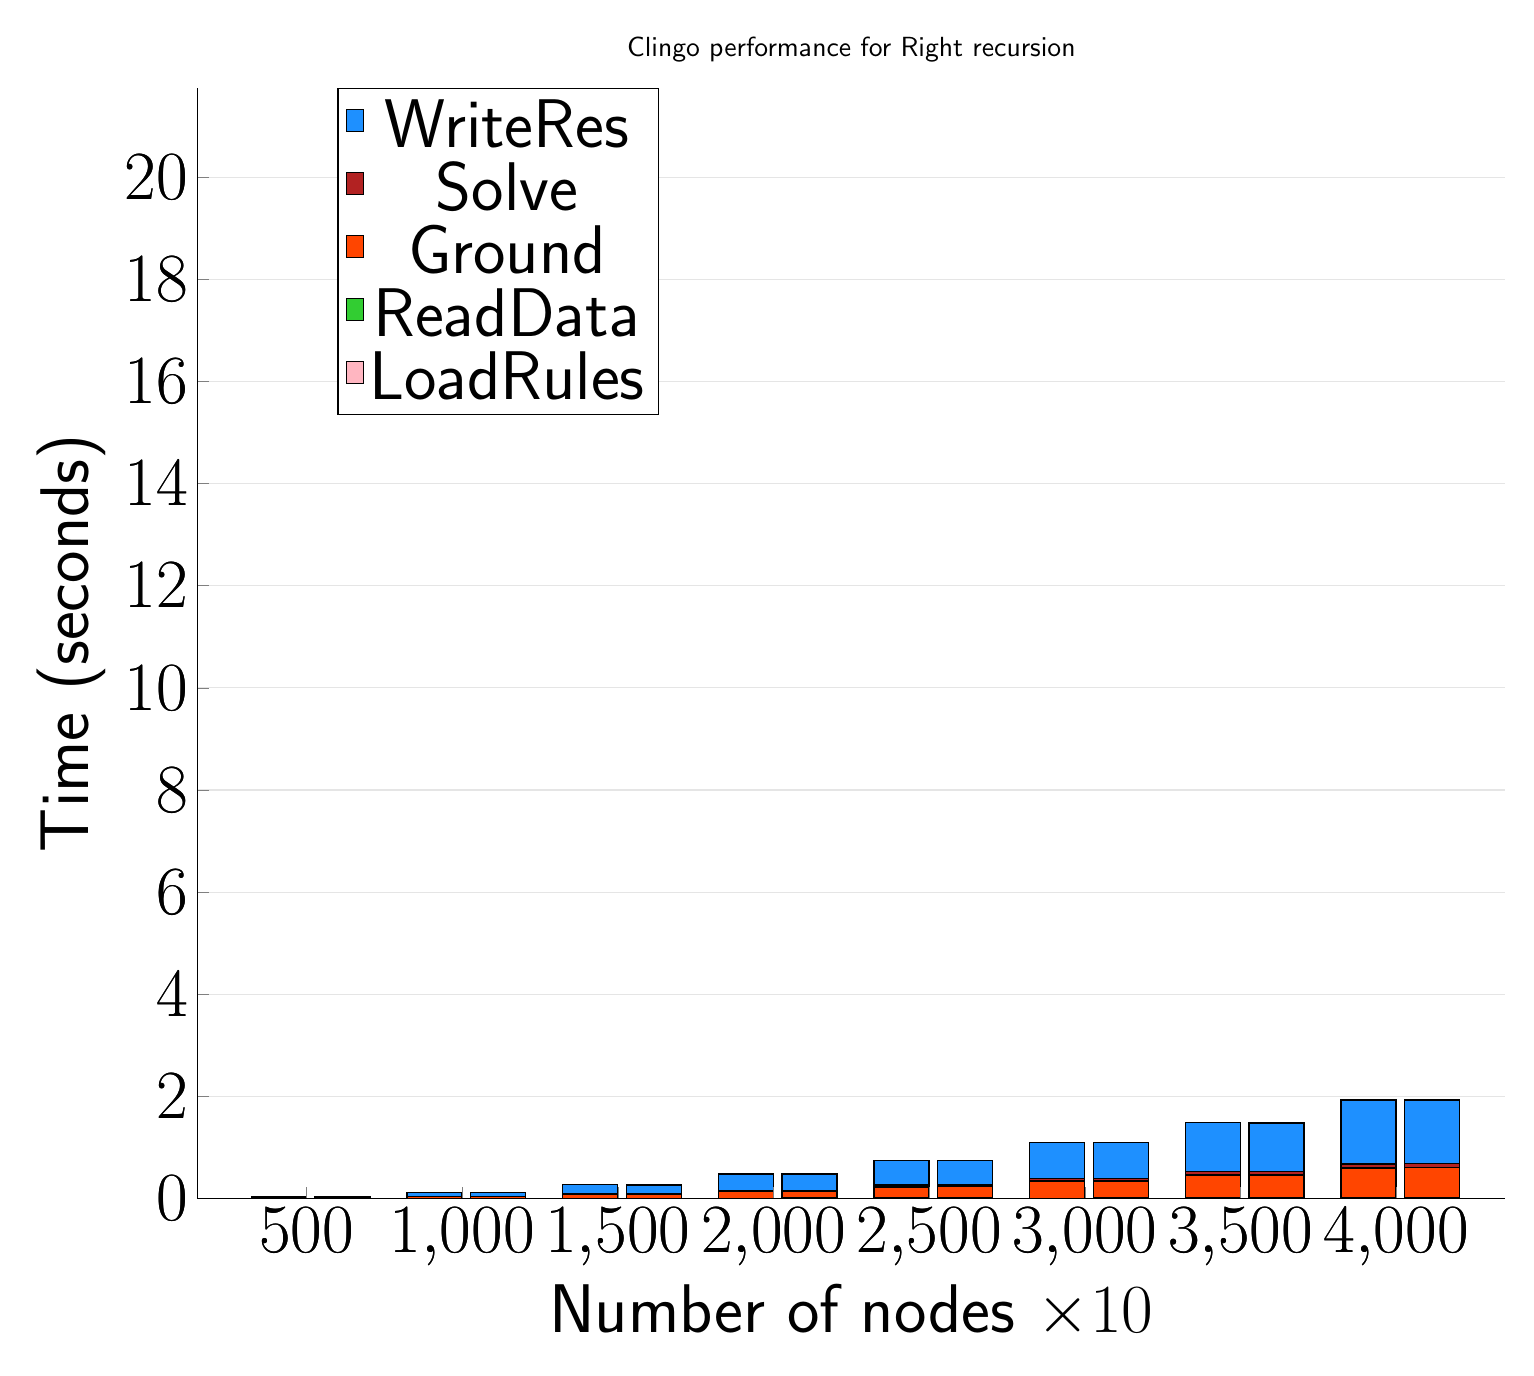
\begin{tikzpicture}
	\begin{axis}[
			ybar stacked,
			title={Clingo performance for Right recursion},
			bar shift=-10pt,
			width=1.5\textwidth,
			bar width=0.7cm,
			ymajorgrids, tick align=inside,
			major grid style={draw=gray!20},
			xtick=data,
			ymin=0, ymax=21.74900002479553,
			axis x line*=bottom,
			axis y line*=left,
			enlarge x limits=0.1,
			legend style={
					at={(0.23, 1)},
					anchor=north,
					legend columns=1,
					font=\Huge,
				},
			ylabel={Time (seconds)},
			xlabel={Number of nodes $\times 10$},
			label style={font=\Huge},
			tick label style={font=\Huge},
		]
		\addlegendimage{fill=DodgerBlue, draw=black, line width=0.2pt}
		\addlegendentry{WriteRes}
		\addlegendimage{fill=FireBrick, draw=black, line width=0.2pt}
		\addlegendentry{Solve}
		\addlegendimage{fill=OrangeRed, draw=black, line width=0.2pt}
		\addlegendentry{Ground}
		\addlegendimage{fill=LimeGreen, draw=black, line width=0.2pt}
		\addlegendentry{ReadData}
		\addlegendimage{fill=LightPink, draw=black, line width=0.2pt}
		\addlegendentry{LoadRules}
		\addplot +[fill=LightPink, draw=black, line width=0.5pt] coordinates {
				(500, 0.0)
				(1000, 0.0)
				(1500, 0.0)
				(2000, 0.0)
				(2500, 0.0009999990463256836)
				(3000, 0.0)
				(3500, 0.0)
				(4000, 0.0)
			};
		\addplot +[fill=LimeGreen, draw=black, line width=0.5pt] coordinates {
				(500, 0.0009999990463256836)
				(1000, 0.0029999971389770507)
				(1500, 0.0019999980926513673)
				(2000, 0.005999994277954101)
				(2500, 0.007999992370605469)
				(3000, 0.0070000171661376955)
				(3500, 0.008999991416931152)
				(4000, 0.009999990463256836)
			};
		\addplot +[fill=OrangeRed, draw=black, line width=0.5pt] coordinates {
				(500, 0.008999991416931152)
				(1000, 0.034999966621398926)
				(1500, 0.07900002002716064)
				(2000, 0.1390000104904175)
				(2500, 0.2210000276565552)
				(3000, 0.33500003814697266)
				(3500, 0.4549999713897705)
				(4000, 0.5910000085830689)
			};
		\addplot +[fill=FireBrick, draw=black, line width=0.5pt] coordinates {
				(500, 0.0009999990463256836)
				(1000, 0.0029999971389770507)
				(1500, 0.01100001335144043)
				(2000, 0.015999984741210938)
				(2500, 0.034999966621398926)
				(3000, 0.04700002670288086)
				(3500, 0.06100001335144043)
				(4000, 0.07899997234344483)
			};
		\addplot +[fill=DodgerBlue, draw=black, line width=0.5pt] coordinates {
				(500, 0.021000003814697264)
				(1000, 0.08299999237060547)
				(1500, 0.17800002098083495)
				(2000, 0.3170000076293945)
				(2500, 0.4820000410079956)
				(3000, 0.7119999885559082)
				(3500, 0.9609999656677246)
				(4000, 1.2520000457763671)
			};
	\end{axis}
	\begin{axis}[
			ybar stacked,
			bar shift=13pt,
			width=1.5\textwidth,
			bar width=0.7cm,
			ymajorgrids, tick align=inside,
			major grid style={draw=none},
			xtick=data,
			ymin=0, ymax=21.74900002479553,
			axis x line*=none,
			axis y line*=none,
			enlarge x limits=0.1,
			label style={font=\Huge},
			tick label style={font=\Huge},
		]
		\addplot +[fill=LightPink, draw=black, line width=0.5pt] coordinates {
				(500, 0.0)
				(1000, 0.0)
				(1500, 0.0)
				(2000, 0.0)
				(2500, 0.0)
				(3000, 0.0)
				(3500, 0.0)
				(4000, 0.0)
			};
		\addplot +[fill=LimeGreen, draw=black, line width=0.5pt] coordinates {
				(500, 0.0)
				(1000, 0.0)
				(1500, 0.0)
				(2000, 0.009999999999999997)
				(2500, 0.009999999999999997)
				(3000, 0.009999999999999997)
				(3500, 0.009999999999999997)
				(4000, 0.009999999999999997)
			};
		\addplot +[fill=OrangeRed, draw=black, line width=0.5pt] coordinates {
				(500, 0.009999999999999997)
				(1000, 0.03999999999999999)
				(1500, 0.07999999999999999)
				(2000, 0.131)
				(2500, 0.22500000000000003)
				(3000, 0.331)
				(3500, 0.4520000000000001)
				(4000, 0.5960000000000001)
			};
		\addplot +[fill=FireBrick, draw=black, line width=0.5pt] coordinates {
				(500, 0.0)
				(1000, 0.0)
				(1500, 0.009999999999999995)
				(2000, 0.017999999999999995)
				(2500, 0.031000000000000028)
				(3000, 0.04700000000000001)
				(3500, 0.06600000000000004)
				(4000, 0.07700000000000004)
			};
		\addplot +[fill=DodgerBlue, draw=black, line width=0.5pt] coordinates {
				(500, 0.020000000000000007)
				(1000, 0.084)
				(1500, 0.17799999999999996)
				(2000, 0.31900000000000006)
				(2500, 0.483)
				(3000, 0.704)
				(3500, 0.95)
				(4000, 1.2489999999999999)
			};
	\end{axis}
\end{tikzpicture}

\end{document}
